%
% File acl2020.tex
%
%% Based on the style files for ACL 2020, which were
%% Based on the style files for ACL 2018, NAACL 2018/19, which were
%% Based on the style files for ACL-2015, with some improvements
%%  taken from the NAACL-2016 style
%% Based on the style files for ACL-2014, which were, in turn,
%% based on ACL-2013, ACL-2012, ACL-2011, ACL-2010, ACL-IJCNLP-2009,
%% EACL-2009, IJCNLP-2008...
%% Based on the style files for EACL 2006 by 
%%e.agirre@ehu.es or Sergi.Balari@uab.es
%% and that of ACL 08 by Joakim Nivre and Noah Smith

\documentclass[11pt,a4paper]{article}
\usepackage[hyperref]{acl2020}
\usepackage{booktabs}
\usepackage{graphicx}
\usepackage{times}
\usepackage{latexsym}
\renewcommand{\UrlFont}{\ttfamily\small}

\usepackage{microtype}

\aclfinalcopy % Uncomment this line for the final submission


\newcommand\BibTeX{B\textsc{ib}\TeX}

\title{Using Natura Language Processing to Identify Unfair Clauses in Terms and Conditions Documents}

\author{Jonathan Sears\\
  Tulane University / New Orleans, LA \\
  \texttt{jsears1@tuane.edu} \\\And
  Nicholas Radwin \\
  Tulane  / New Orleans, LA\\
  \texttt{nradwin@tulane.edu} \\}

\date{}

\begin{document}
\maketitle
\begin{abstract}
Lorem ipsum dolor sit amet, consectetur adipiscing elit, sed do eiusmod tempor incididunt ut labore et dolore magna aliqua. Ut enim ad minim veniam, quis nostrud exercitation ullamco laboris nisi ut aliquip ex ea commodo consequat. Duis aute irure dolor in reprehenderit in voluptate velit esse cillum dolore eu fugiat nulla pariatur. Excepteur sint occaecat cupidatat non proident, sunt in culpa qui officia deserunt mollit anim id est laborum.
\end{abstract}


\section{Introduction}

No one reads Terms and Conditions, but everyone agrees to them. Every online user is faced with these
incredibly dense and complex documents as if they are expected to read them in their entirety before
using a digital tool or app that they want to use. In reality, we just agree to the terms and conditions
to use what's behind them, leaving the user in the dark from the ambiguous, unfair, and even potentially
exploitative clauses that may not be in the user's best interest. 

Our project is focused on bringing these buried, questionable clauses to light so that the user can understand 
what he is agreeing to at a glance. As we experiment wih a variety of learning models, we are building a
summarization tool that takes in terms and conditons as input and generates a page that bullets a list of 
either ambiguous, unfair, or exploitative clauses with a confidence score for how likely the model chose 
those sentences correctly. We also want the tool to highlight the sentences from the orginal text.

\section{Related Work}

Citations within the text appear in parentheses as~\citep{aho1972theory} or, if the author's name appears in the text itself, as \citet{andrew2007scalable}.

1. Claudette
https://arxiv.org/pdf/1805.01217v2.pdf

2. Detecting and explaining unfairness in consumer contracts through memory networks
https://link.springer.com/article/10.1007/s10506-021-09288-2

3. LexGLUE: A Benchmark Dataset for Legal Language Understanding in English
chrome-extension://efaidnbmnnnibpcajpcglclefindmkaj/https://aclanthology.org/2022.acl-long.297.pdf

4. Automatic semantics extraction in law documents
https://dl.acm.org/doi/10.1145/1165485.1165506 

5. When Does Pretraining Help? Assessing Self-Supervised Learning for Law and the CaseHOLD Dataset
https://arxiv.org/abs/2104.08671 Links to an external site. 

\section{Methods}

Lorem ipsum dolor sit amet, consectetur adipiscing elit, sed do eiusmod tempor incididunt ut labore et dolore magna aliqua. Ut enim ad minim veniam, quis nostrud exercitation ullamco laboris nisi ut aliquip ex ea commodo consequat. Duis aute irure dolor in reprehenderit in voluptate velit esse cillum dolore eu fugiat nulla pariatur. Excepteur sint occaecat cupidatat non proident, sunt in culpa qui officia deserunt mollit anim id est laborum.



\section{Results}

Lorem ipsum dolor sit amet, consectetur adipiscing elit, sed do eiusmod tempor incididunt ut labore et dolore magna aliqua. Ut enim ad minim veniam, quis nostrud exercitation ullamco laboris nisi ut aliquip ex ea commodo consequat. Duis aute irure dolor in reprehenderit in voluptate velit esse cillum dolore eu fugiat nulla pariatur. Excepteur sint occaecat cupidatat non proident, sunt in culpa qui officia deserunt mollit anim id est laborum.


Table~\ref{tab:a_table} shows a table. Note that we refer to output generated by \texttt{Experiments.ipynb}. This way, whenever we re-run our notebook, we can regenerate the paper with the latest results.

\begin{table}[ht]
\centering
% note that we can refer to tables generated by our Experiments.ipynb notbook.
\begin{tabular}{rr}
\toprule
    C &    F1 \\
\midrule
  0.1 &  0.90 \\
  1.0 &  0.92 \\
  5.0 &  0.93 \\
 10.0 &  0.89 \\
\bottomrule
\end{tabular}

\caption{\label{tab:a_table} A caption. }
\end{table}

Figure~\ref{fig:a_label} shows a figure

\begin{figure}[ht]
	\centering
	% note that we can refer to figures generated by our Experiments.ipynb notbook.
	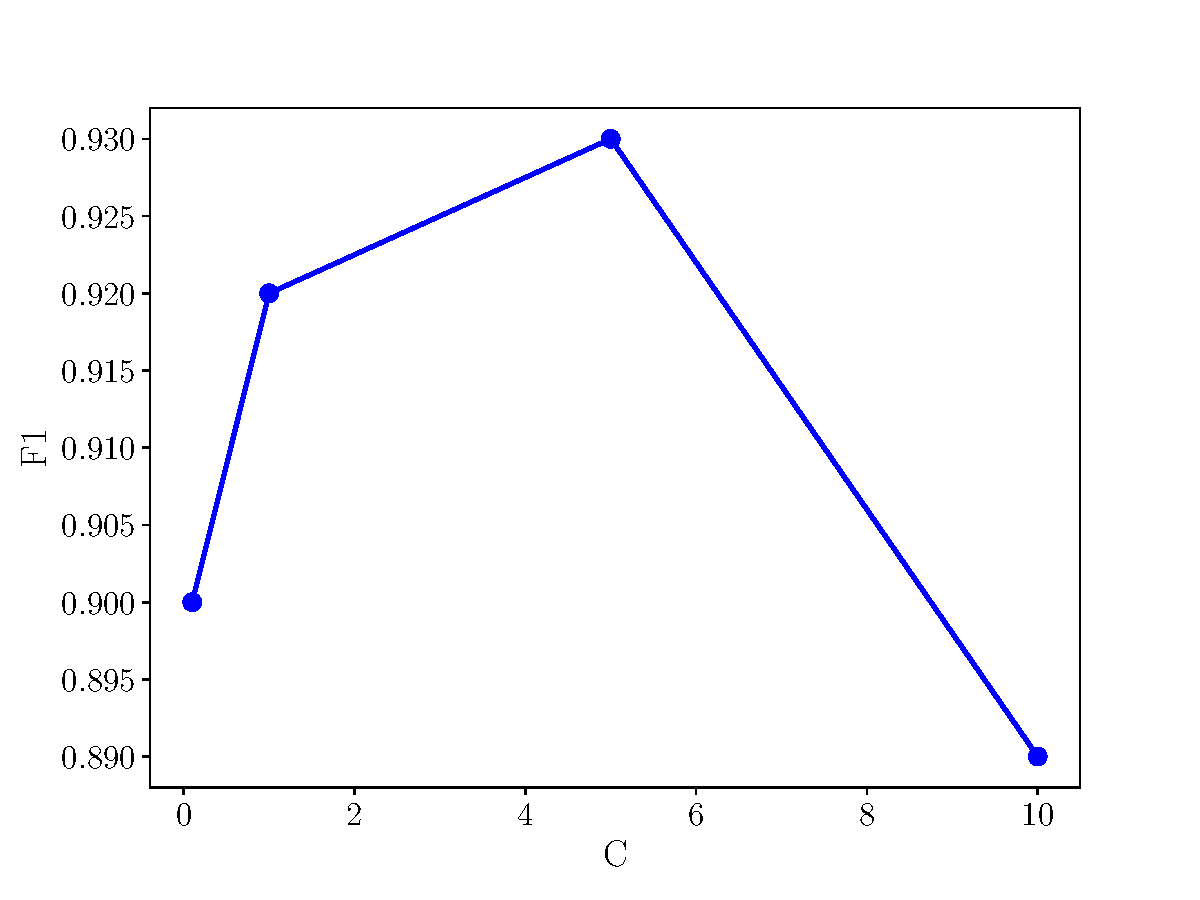
\includegraphics[width=3.5in]{../notebooks/results.pdf}
	\caption{A caption}
	\label{fig:a_label}
\end{figure}

\section{Discussion}

Lorem ipsum dolor sit amet, consectetur adipiscing elit, sed do eiusmod tempor incididunt ut labore et dolore magna aliqua. Ut enim ad minim veniam, quis nostrud exercitation ullamco laboris nisi ut aliquip ex ea commodo consequat. Duis aute irure dolor in reprehenderit in voluptate velit esse cillum dolore eu fugiat nulla pariatur. Excepteur sint occaecat cupidatat non proident, sunt in culpa qui officia deserunt mollit anim id est laborum.


\section{Conclusion}
Lorem ipsum dolor sit amet, consectetur adipiscing elit, sed do eiusmod tempor incididunt ut labore et dolore magna aliqua. Ut enim ad minim veniam, quis nostrud exercitation ullamco laboris nisi ut aliquip ex ea commodo consequat. Duis aute irure dolor in reprehenderit in voluptate velit esse cillum dolore eu fugiat nulla pariatur. Excepteur sint occaecat cupidatat non proident, sunt in culpa qui officia deserunt mollit anim id est laborum.


\section{Division of Labor}
Lorem ipsum dolor sit amet, consectetur adipiscing elit, sed do eiusmod tempor incididunt ut labore et dolore magna aliqua. Ut enim ad minim veniam, quis nostrud exercitation ullamco laboris nisi ut aliquip ex ea commodo consequat. Duis aute irure dolor in reprehenderit in voluptate velit esse cillum dolore eu fugiat nulla pariatur. Excepteur sint occaecat cupidatat non proident, sunt in culpa qui officia deserunt mollit anim id est laborum.





\bibliography{references}
\bibliographystyle{acl_natbib}
@misc{hendersonkrass2022pileoflaw,
  url = {https://arxiv.org/abs/2207.00220},
  author = {Henderson, Peter and Krass, Mark S. and Zheng, Lucia and Guha, Neel and Manning, Christopher D. and Jurafsky, Dan and Ho, Daniel E.},
  title = {Pile of Law: Learning Responsible Data Filtering from the Law and a 256GB Open-Source Legal Dataset},
  publisher = {arXiv},
  year = {2022}
}
@inproceedings{drawzeski-etal-2021-corpus,
  address = {Punta Cana, Dominican Republic},
  author = {Drawzeski, Kasper and Galassi, Andrea and Jablonowska, Agnieszka and Lagioia, Francesca and Lippi, Marco and Micklitz, Hans Wolfgang and Sartor, Giovanni and Tagiuri, Giacomo and Torroni, Paolo},
  booktitle = {Proceedings of the Natural Legal Language Processing Workshop 2021},
  doi = {10.18653/v1/2021.nllp-1.1},
  month = {nov},
  pages = {1--8},
  publisher = {Association for Computational Linguistics},
  title = {{A Corpus for Multilingual Analysis of Online Terms of Service}},
  url = {https://aclanthology.org/2021.nllp-1.1},
  year = {2021}
}
@misc{hendersonkrass2022pileoflaw,
  url = {https://arxiv.org/abs/2207.00220},
  author = {Henderson, Peter and Krass, Mark S. and Zheng, Lucia and Guha, Neel and Manning, Christopher D. and Jurafsky, Dan and Ho, Daniel E.},
  title = {Pile of Law: Learning Responsible Data Filtering from the Law and a 256GB Open-Source Legal Dataset},
  publisher = {arXiv},
  year = {2022}
}

\end{document}
